% Created 2022-06-04 Sat 10:03
% Intended LaTeX compiler: pdflatex
\documentclass[11pt]{article}
\usepackage[utf8]{inputenc}
\usepackage[T1]{fontenc}
\usepackage{graphicx}
\usepackage{longtable}
\usepackage{wrapfig}
\usepackage{rotating}
\usepackage[normalem]{ulem}
\usepackage{amsmath}
\usepackage{amssymb}
\usepackage{capt-of}
\usepackage{hyperref}
\usepackage{cleveref}
\usepackage{subfig}
\usepackage[letterpaper, margin=1in]{geometry}
\usepackage{fancyhdr}
\pagestyle{fancy}
\usepackage{amssymb}
\usepackage{soul}
\usepackage{color}
\usepackage[citestyle=authoryear,bibstyle=authoryear, hyperref=true,backref=true,maxcitenames=3,url=true,backend=biber,natbib=true] {biblatex}
\addbibresource{export/bibs.bib}
\fancyhead[CO,CE]{\textbf{[Align-BDD]}}
\fancyhead[LO,LE]{A.B.}
\fancyhead[RO,RE]{Application: j-UFLP.}
\usepackage{setspace}
\doublespacing
\author{Alexey Bochkarev}
\date{\today}
\title{Align-BDD application: on joint UFLP.}
\hypersetup{
 pdfauthor={Alexey Bochkarev},
 pdftitle={Align-BDD application: on joint UFLP.},
 pdfkeywords={},
 pdfsubject={},
 pdfcreator={Emacs 29.0.50 (Org mode 9.5.2)}, 
 pdflang={English}}
\begin{document}

\maketitle

\section{TBD: Summary and questions}
\label{sec:orgef0e50f}
This section is an internal discussion, while all the rest I hope to include
into the paper draft. Here I tried to get into reviewers'
shoes and try to think critical about what are we trying to present. So, here
are some weak points I would propose to discuss:

\begin{enumerate}
\item \textbf{What worries me most:} I figured CPP MIP is still faster. That is, if I
build BDDs, but skip aligning the diagrams altogether and just solve the CPP
MIP using Gurobi, it just runs way faster. For a specific instance (more or
less representative, as I see it) a naive MIP takes 28 sec, CPP MIP works
below a second, and VS-heuristic needs about 3 sec (to-A baseline takes 5 or
14 sec., depending on what we choose for 'A'). Overall, a naive MIP tends to
be the slowest, alternative alignment heuristics are somewhat faster than
MIP, but slower than our VS-heuristic, and CPP MIP is clearly the fastest.
Maybe that is because the diagrams are small, but this is what I see from my
experiments. It may or may not get better if we try to design instances where
I have still limited, but larger number of connection points between any two
clusters (e.g., no more than 3 arcs between any two clusters). I would need
to modify the algorithm, and I am not sure if that would help, to be honest.
From the other hand, this example just shows: if we are OK with MIP in the
end, we enjoy faster runtimes. With our heuristic, we could compromise some
runtime, but have an LP in the end. I am still not sure if that would count
as a proper response to the reviewers :) although it is indeed best we could
get by this point. A separate question is how to present this carefully, if
we choose to proceed with this problem.
\item Another somewhat weak point (although perhaps it is no different from the
previous one) is that we are feeding more information to the DD-based
methods. Viz., I supply pre-defined data that explicitly says what points are
in which cluster, and what are cluster's connection points. I understand that
this is sort of the whole point, that we are designing a heuristic that would
use additional information that the generic solver doesn't know how to use.
But I wanted to discuss: do you think this comparison is fair? Or rather, how
to describe it in a correct way, so that we wouldn't mislead the reader.
\item I was looking at Figure \ref{fig:sample-jUFLP} and trying to see if I could
just reformulate this problem as a larger UFLP instance (or something along
those lines). It seems I can not, so it is indeed a separate, more complex
problem, right?
\item Finally, I have not that much variety in generated graph topologies: it is
always \(n\) clusters of \(M\) points, the number of edges per cluster is always
the same. I think for \(M=5\) nodes per cluster, it is not that much. I am not
quite sure if this is a problem.
\end{enumerate}

\section{Joint UFLP formulation}
\label{sec:jUFLP}
We next illustrate the performance of our algorithms in the context of a
specific application. In this section we introduce the problem, then discuss a
naive MIP formulation and an alternative CPP approach (where our heuristic can
be used to align the diagrams) in Section \ref{sec:j-UFLP-sol}, and conclude with
numerical experiments in Section \ref{sec:j-UFLP-nums}.

We have designed a problem to highlight a possible application for our
heuristic: It comprises two similar subproblems of special structure, which
makes it natural to represent with BDDs, linked with side constraints implying
the interdependence of some decisions across two subproblems. A subproblem is
the following modification of the uncapacitated facility location problem, UFLP
\citep{owen1998,revelle2008}.

Each of the two subproblems (indexed with \(t=1\) or \(2\)) considers a set of \(N\)
points. At each point \(i\), we can locate a facility at a cost given by \(c^t_i\),
covering all points in a set given by \(S^t_i\), where \(i \in S^t_i\). Set \(S^t_i\)
might refer to customers that are sufficiently close to location \(i\) according
to some specified metric, like distance or travel time. Therefore, the \(N\)
points represent some graph \(G_t\) and \(S^t_i\) encode the respective adjacency
lists. (For convenience, we assume \(G^t\) to be connected.) We also define
overlap cost function \(f^t_i: \mathbb{N}_0\rightarrow\mathbb{R}\), so that
\(f^t_i(a)\) would indicate a cost of covering point \(i\) exactly \(a_i\) times,
within subproblem \(t\). Note that we do not imply any properties of \(f_i\), such
as convexity or concavity. Connection between the subproblems is given by the
condition that there is a set of pairs of points \((i_1, i_2) \in J\) such that
the location decision regarding point \(i_1\) in \(G_1\) must coincide with the
corresponding decision on \(i_2\) in \(G_2\). The problem, which we refer to as
\emph{joint UFLP (j-UFLP)}, minimizes the total cost and can be formulated as follows:

\begin{subequations}\label{eq:j-UFLP}
\begin{align}
  \min & \sum_{i=1, t=1,2}^N \Big(c^t_i x^t_i + f^t_i(a^t_i)\Big)&\\
    \textrm{s.t. } & a^t_i = \sum_{j\in S^t_i} x^t_i& \textrm{ for all } i=1,\ldots, N, t=1,2,\\
    & x^t_i\in\{0,1\} & \textrm{ for all } i=1,\ldots,N, t=1,2,\\
    & x^1_i = x^2_j & \textrm{ for all } (i,j)\in J.\label{eq:link}
\end{align}
\end{subequations}

Further, to make the problem natural to represent with BDDs, we assume that each
sub-problem graph consists of \(n\) subgraphs (\emph{clusters}), \(M\) nodes each, and
that there is at most one arc between every two subgraphs (we refer to the
endpoints of such arcs as \emph{connection points}). Moreover, we assume \(J\) to link
the connection points only. An example of such instance is presented in Figure
\ref{fig:sample-jUFLP}. A subgraph corresponding to the first subproblem, \(G_1\),
is depicted with thick lines, while \(G_2\) is drawn with thin lines. Linking
conditions \eqref{eq:link} imply that some nodes are common in \(G_1\) and \(G_2\).
Such nodes are marked with background color (nodes \texttt{j1}, \texttt{j6}, \texttt{j10}--\texttt{j12},
\texttt{j16}, \texttt{j19}, and \texttt{j21}). Note that overlaps are calculated independently: e.g.,
locating a facility at \texttt{j10} does contribute to \(a_{16}^2\), but not \(a_{16}^1\).

\hl{TBD: ... and after that last sentence I am starting to doubt if
the whole idea of representing the two subproblems on a single graph was good.
Well, there is an arc between \texttt{j10} and \texttt{j16}, but it only "works" when I calculate
overlaps in one subproblem, not in the other one... I feel the need to depict everything in one picture,
but does it makes the exposition easier?}


  \begin{figure}%
    \centering
    \includegraphics[width=\textwidth]{./sample_jUFLP.pdf}%
    \caption{Sample j-UFLP instance graph.}%
    \label{fig:sample-jUFLP}%
\end{figure}

\section{Solution methods}
\label{sec:j-UFLP-sol}
A naive MIP reformulation for \eqref{eq:j-UFLP} implies introducing new binary
variables \(y_{i,a}^t\) indicating whether point \(i\) in subproblem \(t\) was covered
at least \(a\) times:

\begin{subequations}\label{eq:j-UFLP-MIP}
\begin{align}
  \min & \sum_{i=1, t=1,2}^N \Big(c^t_i x^t_i + \sum_{a=1}^{|S_i^t|}q_{i,a}^t y^t_{i,a}\Big)+C&\\
    \textrm{s.t. } & \sum_{a=1}^{|S_i|} y_{i,a}^t = \sum_{j\in S^t_i} x^t_i& \textrm{ for all } i=1,\ldots, N, t=1,2,\\
    & y^t_{i,a} \geq y^t_{i, a+1} & \textrm{ for all }i=1, \ldots, N, t=1,2, a=0,\ldots,|S_i|-1,\\
    & x^t_i\in\{0,1\} & \textrm{ for all } i=1,\ldots,N, t=1,2,\\
    & x^1_i = x^2_j & \textrm{ for all } (i, j)\in J,\label{eq:link-MIP}
\end{align}
\end{subequations}
where \(q_{i,a}=f_i^t(a)-f_i^t(a-1)\) and \(C=\sum_{i,t} f_i^t(0)\) are constants.

From the other hand, such problem can be represented as a CPP with two
fixed-width diagrams (each corresponding to a subproblem), having different
order of variables. For each subproblem, we build a BDD, where a path captures
total cost stemming from the corresponding location decisions in the following
way. We process the clusters in the order we would traverse them without
entering any cluster twice, and add the connection points to the diagram. Note
that when all (at most, four) connection points adjacent to a cluster are added
to the BDD, we can calculate the cost stemming from that cluster by solving at
most four smaller mixed-integer problems. Moreover, in the course of BDD
construction due to the special structure of \(G\) we need to keep track of the
values for at most three variables, which limits the BDD width to \(2^3=8\). This
BDD construction process is illustrated below. Interconnection between
subproblems is achieved by renaming the variables in the diagrams: For each \((i,
j)\in J\) labels of the BDD layers corresponding to \(x_i^1\) and \(x_j^2\) (in the
first and the second BDD, respectively) must coincide.

\textbf{\textbf{Example.}} Let us briefly illustrate the BDD construction procedure for a
single subproblem with Figure \ref{fig:caves}. Assume we have four clusters of
points, denoted \texttt{C1}, \(\ldots\), \texttt{C4} and points \texttt{1}, \(\ldots\), \texttt{6} are
connecting points for these clusters. First, observe that when we fix values for
\(x_1\) and \(x_2\), the costs contribution to the objective stemming from cluster
\texttt{C1} can be obtained by solving a smaller mixed-integer program. The formulation
is similar to \eqref{eq:j-UFLP-MIP}, but with index \(t\) and linking condition
\eqref{eq:link} dropped and the set of nodes restricted to \texttt{C1}. Such MIP would
have only \(M\)  $x_i$-variables, corresponding to \texttt{C1}. Therefore, we
introduce \(x_1\) and \(x_2\) to the BDD and capture the costs stemming from cluster
\texttt{C1} in BDD arc weights. The last new layer would then comprise \(2^2=4\) nodes,
for \((x_1,x_2)\) being equal \((0,0)\), \((1,0)\), \((0,1)\), and \((1,1)\),
respectively. If we further add \(x_3\) and \(x_4\) to the diagram, we can fix costs
stemming from cluster \texttt{C2} in BDD arc costs as well. After we add \(x_3\) the
diagram width increases to \(2^3=8\) (we are keeping track of \(x_1\), \(x_2\), and
\(x_3\)), but after we introduce \(x_4\) we do not need to have \(2^4=16\) nodes in
the last layer. Note that \(x_1\) and \(x_2\) will not affect any costs stemming
from \texttt{C3} and \texttt{C4}. Therefore, BDD nodes corresponding to different values of
these two variables in the last layer can be joined, which would make it
sufficient to have \(x_4\) layer with \(4\) nodes only. Continuing this process, we
build a diagram of width \(2^2=8\) at most (regardless of \(n\) and \(M\)), that
encodes the subproblem. The resulting BDD is presented in Figure
\ref{fig:dcloud-DD}. Because we drop the information regarding specific choices of
\(x_1\) and \(x_2\) the highlighted nodes in Layer 4 will yield only two child nodes
in Layer 5. We indicate selected arc costs in the figure, denoting the objective
for the cluster subproblem \texttt{C1} as \(C1(x_1, x_2)\), for \texttt{C2} as \(C2(x_1, x_2,
x_3, x_4)\), for \texttt{C3} as \(C3(x_3, x_4, x_5, x_6)\), and for \texttt{C4} as \(C4(x_5,
x_6)\). Note that a natural order of variables that allows such compact BDD
representation is determined by the sequence of clusters in the figure (we
processed them from the first to the fourth). Finally, if, for example, we have
another subproblem encoded by a BDD with variables \(x_1^\prime, \ldots,
x_6^\prime\), and \(J=\{(1,6), (2,5), (3,4), (4,3), (5,2), (6,1)\}\), we could
reformulate the j-UFLP as a Consistent Path problem instance by renaming the
variables in the diagram depicted in Figure \ref{fig:dcloud-DD} from \((x_1, x_2,
x_3, x_4, x_5, x_6)\) to \((x^\prime_6, x^\prime_5, x^\prime_4, x^\prime_3,
x^\prime_2, x^\prime_1)\).

  \begin{figure}%
    \centering
    \includegraphics[width=\textwidth]{./caves.pdf}%
    \caption{Sample j-UFLP subproblem graph.\label{fig:caves}}
    \vspace{2em}
    \includegraphics[width=\textwidth]{./dcloud-DD.pdf}%
    \caption{Resulting BDD for the subproblem in Figure \ref{fig:caves}.\label{fig:dcloud-DD}}
\end{figure}

\section{Numerical experiments}
\label{sec:j-UFLP-nums}
We generated approximately 400 instances for each value of \(n\) (number of
clusters), ranging from 5 to 14. Each cluster contained \(M=5\) nodes, with
sparsity parameter \(L=0.25\). The latter implies that during the graph generation
we kept adding edges until the number of randomly generated edges \(|E_k|\) in the
cluster satisfied: $$L > 1 - \frac{|E_k|}{M(M-1) / 2},$$ assuming about one
quarter of all possible \(M(M-1)/2\) edges were not present. We then solved each
instance with each of the two methods:
\begin{itemize}
\item First, we used a naive MIP formulation \eqref{eq:j-UFLP-MIP} (denoted \texttt{MIP} in
the figures below).
\item Second, we built two BDDs as discussed above. The resulting CPP instance was
solved by aligning the diagrams and finding a shortest path between root and
terminal nodes. The diagrams were aligned using the proposed variable-sequence
based heuristic (denoted \texttt{VS-heuristic}) and a simple baseline of aligning the
second diagram to match the order of the first one (denoted \texttt{to A}).
\end{itemize}

The results are presented in Figure \ref{fig:jUFLP-nums}. On the left panel we
present runtimes for each of the solved instances, one point per instance.
Solution time in seconds (logarithmic scale) is along the vertical axis, number
of clusters \(n\) is along the horizontal axis. We see that since we are
leveraging the additional information regarding the composition of the clusters
in the BDD-based approach, VS-based heuristic tends to perform relatively better
than the naive MIP, and this gap increases as the instance size grows. (Numbers
in the rectangles above the lines in the figure indicate the share of instances
where the proposed heuristic were faster than \texttt{MIP} at least by 10\%.) On the
right panel we present histograms of the runtimes for \texttt{MIP} and \texttt{to A}
heuristics, relative to the proposed \texttt{VS-heuristic} for the different numbers of
clusters \(n\). The value of 1.0 (vertical line) implies that the heuristic takes
the same time (for a particular instance) as \texttt{VS-heuristic}. Values to the left
of the vertical line imply the heuristic outperforms the proposed one. We see
that while for \(n=7\) clusters \texttt{VS-heuristic} is almost always slower than MIP,
for larger instances it starts to outperform the baseline on more than two
thirds of the instances.

  \begin{figure}%
    \centering
    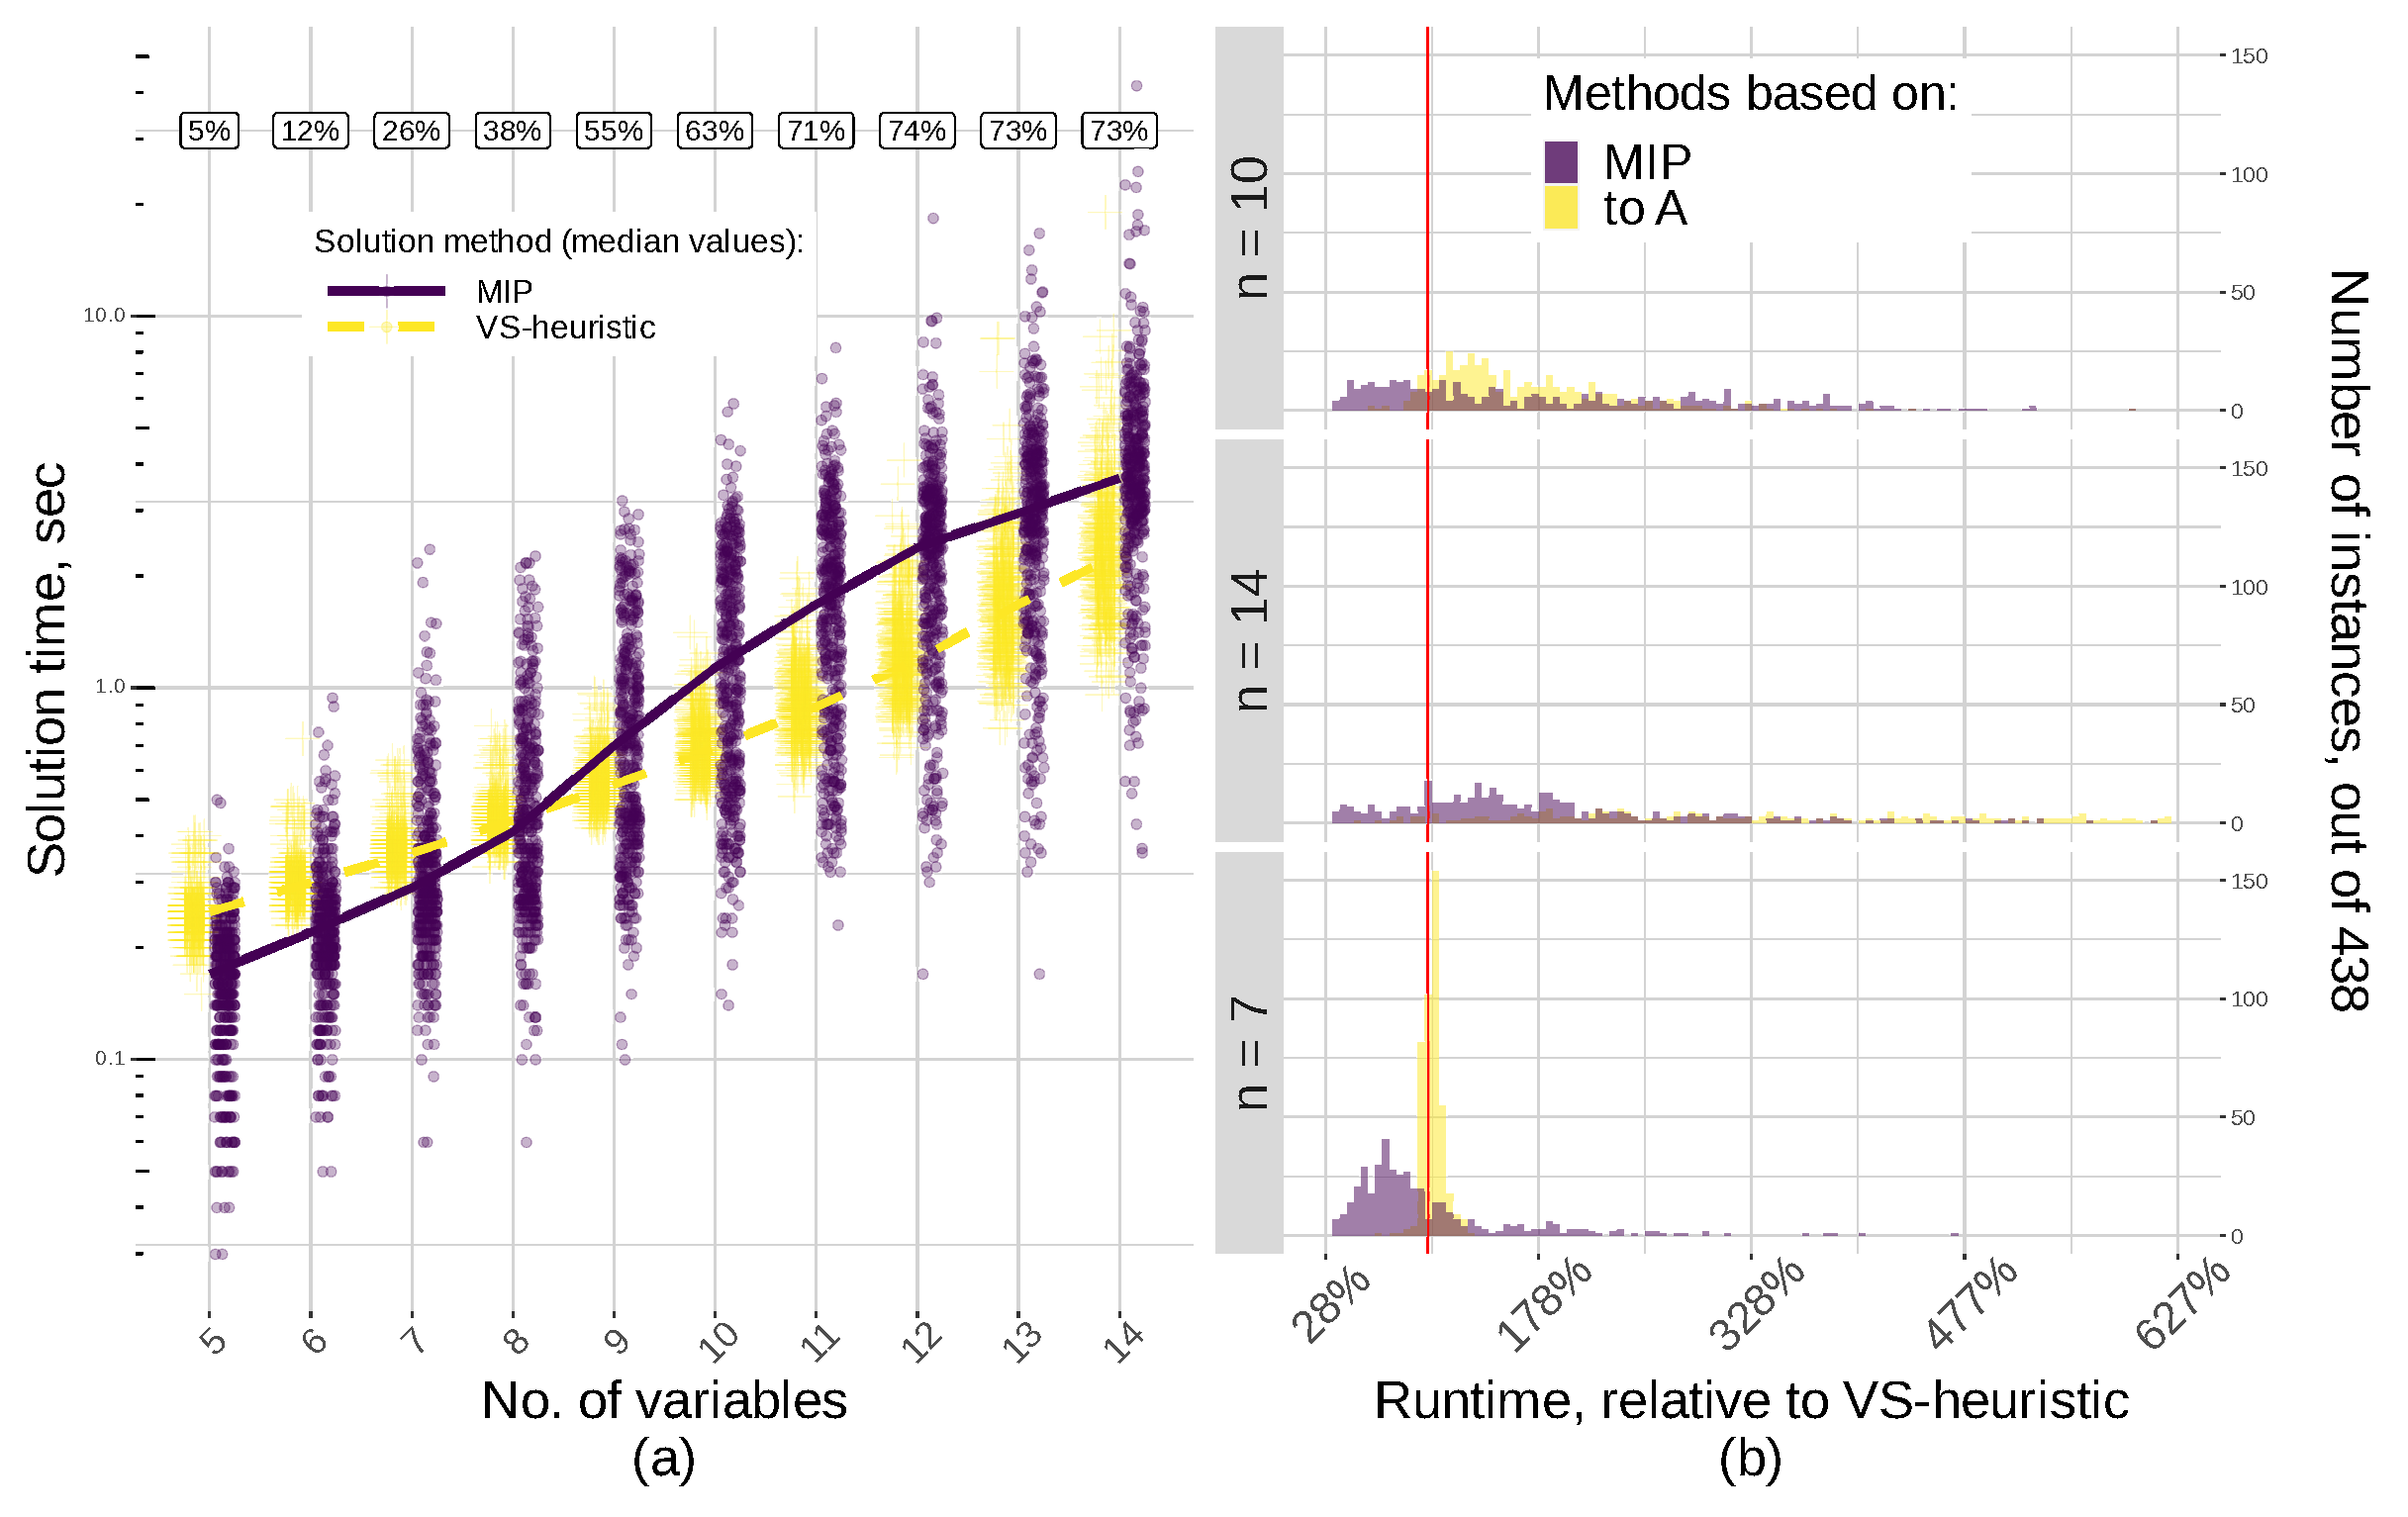
\includegraphics[width=\textwidth]{./jUFLP.eps}%
    \caption{Numerical performance of various heuristics for j-UFLP.}%
    \label{fig:jUFLP-nums}%
\end{figure}

\hl{This is perhaps for Conclusion section:}
This example illustrates a possible way to reformulate a complex combinatorial
problem as a large LP. When such problem possesses a special structure that
makes it natural to represent with a collection of BDDs with different order of
variables, we can try to align these BDDs to build an intersection and formulate
a shortest-path in the intersection BDD. The heuristic we propose in many cases
allows to find a good shared variable order for the diagrams and avoid costly
manipulations with decision diagrams directly.
\printbibliography
\end{document}